 \chapter{Feldtheoretische Beschreibung von Wellenleitern}
Die Ausbreitung von Wellen im Freiraum wurde bereits betrachtet. Für technische Anwendungen ist es mitunter hilfreich, Wellen entlang einer führenden Struktur zu transportieren. Diese Struktur nennt man dann \textbf{Wellenleiter}. Es gibt viele Formen von \textbf{Wellenleitern} in technischer Nutzung. Beispiele sind:
	\begin{center}
		\resizebox{\textwidth}{!}{
\begin{minipage}{.25\linewidth}
	\centering
	Hohlleiter
	\bigskip

	\def\r{1.8}
	\tdplotsetmaincoords{70}{120}
	\begin{tikzpicture}[tdplot_main_coords]
		% Drawing XYZ coordinates system
		\def \lenX {1.0*\r}
		\def \lenY {1.0*\r}
		\def \lenZ {0.3*\r}
		\def \boxX{.7*\r}
		\def \boxY{.9*\r}
		\def \boxZ{.2*\r}
		% Calculate box corner length
		\pgfmathsetmacro{\boxCornerLen}{sqrt{((\boxX)^2 + (\boxY)^2 + (\boxZ)^2)}}
		% Draw coordinate system
		\draw[dashed] (0,0,0) -- (\boxX,0,0);
		\draw[-stealth,thin] (\boxX,0,0) -- (\lenX,0,0) node[left] {$y$};
		\draw[dashed] (0,0,0) -- (0,\boxY,0);
		\draw[-stealth,thin] (0,\boxY,0) -- (0,\lenY,0) node[anchor=north west] {$z$};
		\draw[dashed] (0,0,0) -- (0,0,\boxZ);
		\draw[-stealth,thin] (0,0,\boxZ) -- (0,0,\lenZ) node[anchor=south] {$x$};

		% Drawing horizontal box:
		% Get corner polar coordinate
		\tdplotgetpolarcoords{\boxX}{\boxY}{\boxZ}
		\tdplotsetcoord{Box}{\boxCornerLen}{\tdplotrestheta}{\tdplotresphi}
		% Draw a box
		\draw[] (Boxx) -- (Boxxy);
		\draw[very thick] (Boxy) -- (Boxxy);
		\draw[] (Boxx) -- (Boxxz);
		\draw[] (Boxz) -- (Boxxz);
		\draw[very thick] (Boxy) -- (Boxyz);
		\draw[] (Boxz) -- (Boxyz);
		\draw[very thick] (Boxxy) -- (Box);
		\draw[] (Boxxz) -- (Box);
		\draw[very thick] (Boxyz) -- (Box);
	\end{tikzpicture}

\end{minipage}
\begin{minipage}{.25\textwidth}
	\centering
	Koaxialkabel

	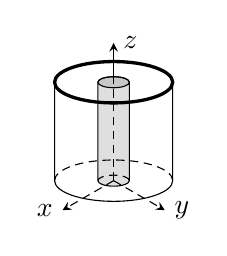
\begin{tikzpicture}
		\draw [fill=gray, fill opacity=.25] (180:2mm) coordinate (a)
		-- ++(0,-12.5mm) coordinate (b)
		arc (180:360:2mm and .7mm) coordinate (d) % 2 war 5
		-- (a -| d) coordinate (c) arc (0:180:2mm and .7mm); % 2 war 5
		\draw [fill=gray, fill opacity=.25]
		(0,0) coordinate (t) circle (2mm and .7mm);
		\draw [densely dashed] (d) arc (0:180:2mm and .7mm);
		\draw []
		(180:7.5mm) coordinate (A)
		-- ++(0,-12.5mm) coordinate (B)
		arc (180:360:7.5mm and 2.625mm) coordinate (D)
		-- (A -| D) coordinate (C) arc (0:180:7.5mm and 2.625mm);
		\draw [very thick]
		(0,0) coordinate (T) circle (7.5mm and 2.625mm);
		\draw [densely dashed] (D) arc (0:180:7.5mm and 2.625mm);
		\draw [densely dashed ]
		([yshift=-12.5mm]T) coordinate (B)
		edge [-stealth] node [pos=1, right] {$y$} +(-30:7.5mm)
		edge [-stealth] node [pos=1, left] {$x$} +(-150:7.5mm)
		-- (T) edge [solid, -stealth] node [right, pos=1] {$z$} ++(0,5mm) ;
	\end{tikzpicture}

\end{minipage}
\begin{minipage}{.25\textwidth}
	\centering
	Zweidrahtleitung (Lecher-Leitung)

	\begin{tikzpicture}
		\node [thick,cylinder, draw, shape border rotate=90,minimum height=1.5cm,minimum width=2mm] at (0,0){};
		\node [thick,cylinder, draw, shape border rotate=90,minimum height=1.5cm,minimum width=2mm] at (1cm,0cm){};
		\draw[thin, -stealth] (0.5cm,-0.80cm) -- (0.5cm,1cm) node[above]{$z$};
	\end{tikzpicture}
\end{minipage}
\begin{minipage}{.25\textwidth}
	\centering
	Mikrostreifenleitung
	\bigskip

	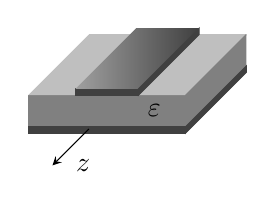
\begin{tikzpicture}[scale=0.4]
		\draw [lightgray] (0,1,0) coordinate (bl) -- (5,1,0) coordinate (br);
		\filldraw [gray] (0,0,5) coordinate (fll) -- (0,1,5) coordinate (ftl) -- (5,1,5) coordinate (ftr) -- (5,0,5) coordinate (flr) -- cycle;
		\shade [left color = lightgray, right color = lightgray] (bl) -- (br) -- (ftr) -- (ftl) -- cycle;
		\filldraw [gray] (5,0,0) coordinate (blr) -- (flr) -- (ftr) -- (br);
		\filldraw [darkgray] (fll) rectangle (5,-0.2,5) coordinate (flr2);
		\filldraw [darkgray] (flr2) -- (5,-0.2,0) coordinate (blr2) -- (blr) -- (flr) -- cycle;
		\filldraw [darkgray] (1.5,1.2,5) coordinate (ftl-1) -- (3.5,1.2,5) coordinate (ftr-1) -- (3.5,1,5) coordinate (flr-1) -- (1.5,1,5) coordinate (fll-1) -- cycle;
		\shade [left color = darkgray!50, right color = darkgray] (1.5,1.2,0) coordinate (btl-1) -- (3.5,1.2,0) coordinate (btr-1) -- (ftr-1) -- (ftl-1) -- cycle;
		\filldraw [darkgray] (flr-1) -- (ftr-1) -- (btr-1) --  (br -| btr-1) -- cycle;
		\node at (4,0.5,5) {$\varepsilon$};
		\coordinate (nA1) at (1.5,2.5,0);
		\coordinate (nB1) at (3.5,2.5,0);
		\coordinate (nA2) at (-1.5,1.2,0);
		\coordinate (nB2) at (-1.5,1.2,5);
		\coordinate (nA3) at (7,1,5);
		\coordinate (nB3) at (7,1.2,5);
		\coordinate (nA4) at (-1.5,1,5);
		\coordinate (nB4) at (-1.5,0,5);
		\draw[-stealth,thin] (0,-2,0) -- (0,-2,3) node[right,xshift=5]{$z$};
	\end{tikzpicture}

\end{minipage}}
	\end{center}
	\section{Abgrenzung der Betrachtung}
	In dem Kapitel \enquote{Feldtheoretische Beschreibung von Wellenleitern} werden nur (1) \textbf{zylindrische Wellenleiter} mit (2) \textbf{metallischen Begrenzungen} bei (3) \textbf{harmonischer Zeitabhängigkeit} betrachtet. Es gibt allgemein zwei Herangehensweisen zur Beschreibung von Wellenleitern, einmal die \textbf{feldtheoretische} (in diesem Abschnitt) und die \textbf{Leitungstheorie} (mit Strom und Spannung, siehe \ref{leitungstheorie}).
	\subsection{Zylindrische Wellenleiter}
	 Alle hier betrachteten Strukturen sind in $z$-Richtung (eine beliebige Richtung, Koordinatensystem ggf. passend hindrehen) \textbf{translationsinvariant}. Es sind alle Schnitte senkrecht zu $z$ identisch. In diesem Fall wird von \textbf{zylindrischen Wellenleitern} gesprochen (auch bei Nicht-Kreiszylindern). Das Lösungsgebiet ist ein lineares, homogenes und isotropes Dielektrikum mit den Parametern \(\varepsilon\) und \(\mu\). Alles andere ist ein perfekter Leiter (\(\kappa \to \infty\)). 
	 \begin{center}
	 	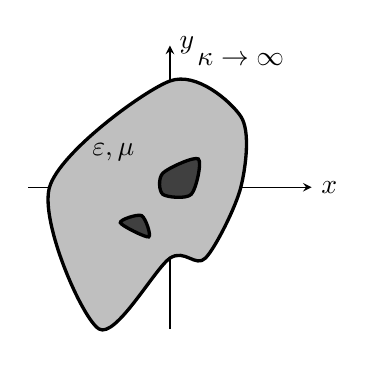
\begin{tikzpicture}[scale=.9]
	\draw [thin, -stealth] (-2,0) -- (2,0) node[right]{$x$};
	\draw [thin, -stealth] (0,-2) -- (0,2) node[right]{$y$};
	\draw [very thick, draw=black, fill=lightgray] plot [smooth cycle] coordinates {(-1,-2) (-1.7,0) (0,1.5) (1,1) (1,0) (0.5,-1) (0,-1)};
	\draw [very thick, fill=darkgray] plot [smooth cycle] coordinates {(-.7,-.5) (-.4,-.4) (-.3,-.7)};
	\draw [very thick, fill=darkgray] plot [smooth cycle] coordinates {(-.1,-.1) (-.1,.2) (0.4,0.4) (.3,-.1)};
	\node at (1,1.8){$\kappa\to\infty$};
	\node at (-.8,.5){$\varepsilon,\mu$};
\end{tikzpicture}
	 \end{center}
	 Die Vektoren \(\vu{x}\) und \(\vu{y}\) spannen die \textbf{Querschnittebene} oder \textbf{Transversalebene} auf. Die genaue Geometrie ist aber bis auf die Translationsinvarianz in $z$-Richtung egal.    
	 \subsection{Metallische Begrenzung}
	 Hier werden nur Wellenleiter mit \textbf{metallischen Begrenzungen} betrachtet. Es existieren auch dielektrische Wellenleiter (basierend auf dem Prinzip der Totalreflexion), welche hier aber nicht näher betrachtet werden sollen. Reflexionen (und dadurch eine Führung) treten auch bei metallischen Wellenleitern auf. Man könnte als Lösungsansatz (für eine analytische Beschreibung der Felder im Leiter) die Welle im Zeitbereich mit all ihren Reflexionen überlagern und würde die selbe \textbf{stationäre Lösung} erhalten wie in diesem Abschnitt über den Weg im Frequenzbereich, die transiente Lösung geht durch den Weg über Phasoren aber verloren.
\subsection{Harmonische Zeitabhängigkeit (Helmholtz-Gleichung)}
Es wird der Fall \textbf{harmonischer Zeitabhängigkeit} analysiert (diese ist weiterhin keine Einschränkung, weil man eine Fourier-Synthese durchführen kann). Die homogene Wellengleichung ($\nearrow$\ref{homwell}) wird dadurch zur \textbf{Helmholtz-Gleichung} im Frequenzbereich (Phasoren, \(\mathrm{j}\omega\) statt $\frac{\partial}{\partial t}$):
	\begin{align}
		\square \ubar{\vec{E}}(\vec{r} , t) = \left(\Delta - \varepsilon\mu\frac{\partial^2}{\partial t^2}\right) \ubar{\vec{E}} (\vec{r} , t) = \vec{0} &  & \rightarrow &  & \left(\Delta + \varepsilon\mu\omega^2\right) \ubar{\vec{E}}(\vec{r} ) =\vec{0} \label{helmholtze} \\
		\square \vec{\ubar{B}}(\vec{r} , t) = \left(\Delta - \varepsilon\mu\frac{\partial^2}{\partial t^2}\right) \vec{\ubar{B}} (\vec{r} , t) = \vec{0} &  & \rightarrow &  & \left(\Delta + \varepsilon\mu\omega^2\right) \vec{\ubar{B}}(\vec{r} ) =\vec{0}\label{helmholtzb}
	\end{align}
	Die Gleichungen können im Leiter bzw. im Dielektrikum analog mit einer komplexen Permittivität formuliert werden, wobei dadurch ein Dämpfungsterm entsteht bzw. Verluste auftreten.
\section{Zerlegung von Gesetzen, Operatoren und Vektoren}
Die Translationsinvarianz kann dahingehend genutzt werden, dass Vektoren und Operatoren zerlegt werden können.
\subsection{Zerlegung von Feldstärke- und Flussdichtevektor}
\begin{center}
	\input{res/VKZ}
\end{center}
  Jeder Vektor kann immer in eine \textbf{transversale} und eine \textbf{longitudinale} Komponente zerlegt werden:
	\begin{equation}\label{vekzerl}\begin{split}
			\textcolor{red}{\ubar{\vec{E}}} &= \textcolor{green}{\ubar{\vec{E}}_t} + \textcolor{blue}{\ubar{\vec{E}}_z} = \textcolor{green}{\ubar{\vec{E}}_t} + \textcolor{blue}{\ubar{E}_z\vu{z}} \\
			\textcolor{green}{\ubar{\vec{E}}_t} &= \textcolor{green}{(\vu{z}\times\ubar{\vec{E}})\times\vu{z}}
	\end{split}\end{equation}
 Diese Zerlegung funktioniert analog für magnetische Flussdichte.
	\subsection{Zerlegung des Induktions- und Durchflutungsgesetzes}
		\subsubsection{Longitudinale Komponente des Induktionsgesetzes}
	  Magnetische Flussdichte und elektrisches Feld sind über \ref{ind} verkoppelt (\(\rot \ubar{\vec{E}} = -\mathrm{j}\omega\vec{\ubar{B}}\)). In kartesischen Koordinaten gilt für die Rotation:
	\begin{equation}\begin{split}
			\rot \vec{F} &= \left[ \frac{\partial F_{z}}{\partial y} - \frac{\partial F_{y}}{\partial z} \right] \vu{x} + \left[ \frac{\partial F_{x}}{\partial z} - \frac{\partial F_{z}}{\partial x} \right] \vu{y } + \left[ \frac{\partial F_{y}}{\partial x} - \frac{\partial F_{x}}{\partial y}\right] \vu{z} \\
			&=\nabla \times \vec{F} = \left[ \frac{\partial}{\partial x}\vu{x} + \frac{\partial}{\partial y}\vu{y} + \frac{\partial}{\partial z}\vu{z}\right] \times \vec{F}
	\end{split}\end{equation}
	Es wird die \textbf{transversale Rotation} definiert:
	\begin{equation}\label{transvrot}\begin{split}
			\rot _t & = \nabla_t \times := (\nabla - \frac{\partial}{\partial z} \vu{z}) \times\\
			\rot _t \vec{F} &= \nabla_t \times \vec{F} = \left[ \frac{\partial}{\partial x}\vu{x} + \frac{\partial}{\partial y}\vu{y} + 0\, \vu{z}\right] \times \vec{F}\\
			&=  \left[ \frac{\partial F_{z}}{\partial y} \right] \vu{x} + \left[ - \frac{\partial F_{z}}{\partial x} \right] \vu{y } + \left[ \frac{\partial F_{y}}{\partial x} - \frac{\partial F_{x}}{\partial y}\right] \vu{z}
	\end{split}\end{equation}
	 Offenbar stimmen die \textbf{longitudinalen Anteile} (\(z\)-Komponente) überein, d.h. es gilt:
	\begin{equation}
		\vu{z} \cdot \left(\rot _t \vec{F}\right) = \vu{z} \cdot \rot \vec{F}
	\end{equation}
	 Angewendet auf die \(z\)-Komponente des Induktionsgesetzes bedeutet das:
	\begin{equation}\label{longind}
		\vu{z} \cdot \left(\rot _t \ubar{\vec{E}}\right)=\vu{z} \cdot \left(\rot _t \ubar{\vec{E}}_t + \rot _t \ubar{\vec{E}}_z\right) =\boxed{\vu{z} \cdot \left(\rot _t \ubar{\vec{E}}_t\right) = -\mathrm{j}\omega\ubar{B}_z}
	\end{equation}
\subsubsection{Transversale Komponente des Induktionsgesetzes}
	 Für die transversalen Komponenten gilt entsprechend \ref{vekzerl}:
	\begin{align}
		(\vu{z}\times\rot \ubar{\vec{E}})\times\vu{z}                                                                                                                                                                         & = (\vu{z}\times(-\mathrm{j}\omega\vec{\ubar{B}}))\times\vu{z}                                                                     \nonumber\\
		\left[ \frac{\partial \ubar{E}_{z}}{\partial y} - \frac{\partial \ubar{E}_{y}}{\partial z} \right] \vu{x} + \left[ \frac{\partial \ubar{E}_{x}}{\partial z} - \frac{\partial \ubar{E}_{z}}{\partial x} \right] \vu{y} & = -\mathrm{j}\omega \left(\ubar{B}_x \vu{x} + \ubar{B}_y \vu{y} \right) = -\mathrm{j}\omega \vec{\ubar{B}}_t \;\;|\; \vu{z}\times \nonumber\\
		\left[ \frac{\partial \ubar{E}_{z}}{\partial y} - \frac{\partial \ubar{E}_{y}}{\partial z} \right] \vu{y} - \left[ \frac{\partial \ubar{E}_{x}}{\partial z} - \frac{\partial \ubar{E}_{z}}{\partial x} \right] \vu{x} & = -\mathrm{j}\omega \vu{z}\times \vec{\ubar{B}}_t                                                                                 \nonumber\\
		\left[ \frac{\partial \ubar{E}_{z}}{\partial x} \vu{x} + \frac{\partial \ubar{E}_{z}}{\partial y} \vu{y} \right] - \frac{\partial}{\partial z}\left(\ubar{E}_{x}\vu{x} + \ubar{E}_{y}\vu{y} \right)                   & = -\mathrm{j}\omega \vu{z}\times \vec{\ubar{B}}_t                                                                                 \nonumber\\
		\Aboxed{\grad _t \ubar{E}_{z} - \frac{\partial}{\partial z}\ubar{\vec{E}}_t                                                                                                                                           & = -\mathrm{j}\omega \vu{z}\times \vec{\ubar{B}}_t} \label{transind}
	\end{align}
	Dabei wird offensichtlich der \textbf{transversale Gradient} definiert:
	\begin{equation}
		\grad_t=\nabla_t:= \nabla-\frac{\partial }{\partial z} \vu{z}=\left[ \frac{\partial }{\partial x} \vu{x} + \frac{\partial }{\partial y} \vu{y} \right]
	\end{equation}
\subsubsection{Transversale und longitudinale Komponente des Durchflutungsgesetzes}
	 Aus dem Durchflutungsgesetz ($\nearrow$\ref{durchf} mit $J=0$), also \(\rot \vec{\ubar{B}} = \mathrm{j}\omega\varepsilon\mu\ubar{\vec{E}}\) folgt analog:
	\begin{align}
		\Aboxed{\vu{z} \cdot \left(\rot _t \vec{\ubar{B}}_t\right) &= \mathrm{j}\omega\varepsilon\mu\ubar{E}_z} \label{longdurchf} \\
		 \Aboxed{\grad _t \ubar{B}_{z} - \frac{\partial}{\partial z}\vec{\ubar{B}}_t& = \mathrm{j}\omega\varepsilon\mu \vu{z}\times \ubar{\vec{E}}_t} \label{transdurchf}
	\end{align}

\subsection{Bestimmung der transversalen Komponenten der Vektoren}
	Die transversalen Komponenten \ref{transind} und \ref{transdurchf}
	können entkoppelt werden. Je nachdem, ob die Welle hinlaufend (-) oder rücklaufend (+) ist, gilt: \(\frac{\partial \ubar{E}_z}{\partial z} = \mp \mathrm{j} k \ubar{E}_z\). Außerdem gilt immer \(\frac{\partial^2 \ubar{E}_t}{\partial z^2} = -  k^2 \ubar{E}_t\). Damit folgt nun: 
	\begin{equation}\begin{split}
		&\grad _t \frac{\partial}{\partial z}\ubar{B}_{z} - \frac{\partial}{\partial z}\left(\frac{\partial}{\partial z}\vec{\ubar{B}}_t\right) = \mathrm{j}\omega\varepsilon\mu \vu{z}\times \frac{\partial}{\partial z}\ubar{\vec{E}}_t\\
		\Rightarrow \quad &k^2 \vec{\ubar{B}}_t = -\grad _t \frac{\partial}{\partial z}\ubar{B}_{z}+\mathrm{j}\omega\varepsilon\mu \vu{z}\times \frac{\partial}{\partial z}\ubar{\vec{E}}_t\\
		\text{analog: } \quad &\ubar{\vec{E}}_t =-\frac{1}{k^2}\grad _t \frac{\partial}{\partial z}\ubar{E}_{z}-\frac{1}{k^2}\mathrm{j}\omega \vu{z}\times \frac{\partial}{\partial z}\ubar{\vec{B}}_t\\
		\Rightarrow \quad &\vec{\ubar{B}}_t = -\frac{1}{k^2}\grad _t \frac{\partial}{\partial z}\ubar{B}_{z}\\&\quad\quad\quad+\frac{1}{k^2}\mathrm{j}\omega\varepsilon\mu \vu{z}\times \frac{\partial}{\partial z}\left(-\frac{1}{k^2}\grad _t \frac{\partial}{\partial z}\ubar{E}_{z}-\frac{1}{k^2}\mathrm{j}\omega \vu{z}\times \frac{\partial}{\partial z}\ubar{\vec{B}}_t\right)\\
		\Rightarrow \quad &\vec{\ubar{B}}_t = \pm \frac{\mathrm{j}}{k}\grad _t\ubar{E}_{z}+\frac{1}{k^2}\mathrm{j}\omega\varepsilon\mu \vu{z}\times \left(\grad _t \ubar{E}_{z}+\mathrm{j}\omega \vu{z}\times \ubar{\vec{B}}_t\right)\\
		\stackrel{\text{\ref{grass}}}{\Rightarrow} \quad &\ubar{\vec{B}}_t = \pm \frac{\mathrm{j}}{k}\grad _t\ubar{E}_{z}+\frac{\mathrm{j}}{k^2}\omega\varepsilon\mu \vu{z} \times\grad _t \ubar{E}_{z}+\frac{\mathrm{1}}{k^2}\omega^2\varepsilon\mu  \ubar{\vec{B}}_t\\
		\Rightarrow \quad & \vec{\ubar{B}}_t(k^2-\omega^2\varepsilon\mu)=\pm \mathrm{j}k\grad _t\ubar{E}_{z}+\mathrm{j}\omega\varepsilon\mu \vu{z} \times\grad _t \ubar{E}_{z}\\
		\Rightarrow \quad & \vec{\ubar{B}}_t = \frac{\mathrm{j}}{\omega^2\varepsilon\mu-k^2}\left[\mp k\grad _t\ubar{E}_{z}-\omega\varepsilon\mu \vu{z} \times\grad _t \ubar{E}_{z} \right]
	\end{split}\end{equation}
	 $E_t$ lässt sich analog berechnen. Es ist zu beachten, dass im TEM-Fall ($E_z=0$, \ref{disp}$\Rightarrow k^2-\omega^2\varepsilon\mu=0$) die letzte Division nicht zulässig ist. Die Gleichung ist durch $0=0$ bereits davor erfüllt. Die entkoppelten Gleichungen lauten zusammengefasst:
	\begin{equation}\label{entkoppelgl}\begin{split}
			\Aboxed{\ubar{\vec{E}}_t &= \frac{\mathrm{j}}{\omega^2\varepsilon\mu -  k^2} \left[ \mp  k\, \grad _t \ubar{E}_{z} + \omega  \vu{z}\times\grad _t \ubar{B}_{z}\right]}\\
			\Aboxed{\vec{\ubar{B}}_t &= \frac{\mathrm{j}}{\omega^2\varepsilon\mu -  k^2} \left[ \mp  k\, \grad _t \ubar{B}_{z} - \omega\varepsilon\mu  \vu{z}\times\grad _t \ubar{E}_{z}\right]}
	\end{split}\end{equation}
	Sind die \textbf{longitudinalen Feldkomponenten bekannt}, so lassen sich die \textbf{transversalen Feldkomponenten berechnen}. Im Allgemeinen ist es schwierig, die longitudinalen Komponenten zu finden, aber es gibt einfache Spezialfälle. 
\subsection{Helmholtz-Gleichungen mit transversalem Laplace-Operator}
	Der Laplace-Operator kann in kartesischen Koordinaten \((x,y,z)\) folgendermaßen zerlegt werden, wobei ein \textbf{transversaler Laplace-Operator} definiert wird:
	\begin{equation}\begin{split}
			\Delta &= \underbrace{\frac{1}{\rho}\frac{\partial }{\partial \rho}\left(\rho\frac{\partial }{\partial \rho}\right)+\frac{1}{\rho^{2}}\frac{\partial^{2}}{\partial \varphi^{2}}}_{:=\Delta _t}+\frac{\partial^{2}}{\partial z^{2}} = \Delta _t + \frac{\partial^{2}}{\partial z^{2}}\\
			\Delta &= \underbrace{\frac{\partial^2}{\partial x^2}+\frac{\partial^2}{\partial y^2}}_{:=\Delta _t}+\frac{\partial^2}{\partial z^2} = \Delta _t + \frac{\partial^{2}}{\partial z^{2}}
	\end{split}\end{equation}
	 Zur Lösung der Helmholtzgleichungen ($\nearrow$\ref{helmholtze},\ref{helmholtzb})
	wird eine \textbf{in \(z\)-Richtung propagierende Welle} angesetzt (hier beispielhaft nur für $E$):
	\begin{equation}
		\ubar{\vec{E}}(\vec{r} , t) = \ubar{\vec{E}}_0(x,y)  \mathrm{e}^{\mathrm{j}(\omega t \pm  k z)} \stackrel{\text{ruhender Zeiger}}{\to}  \ubar{\vec{E}}(\vec{r} ) = \ubar{\vec{E}}_0(x,y)  \mathrm{e}^{\pm\mathrm{j} k z}
	\end{equation}
$\ubar{\vec{E}}_0(x,y)$ kann keine $z$-Abhängigkeit haben, sonst würde es Probleme bei der Erfüllung der Wellengleichung geben, wenn diese unter Einhaltung harmonischer Zeitabhängigkeit erfüllt werden soll. Wenn mit diesem Ansatz eine Lösung erhalten wird, die die Randbedingungen erfüllt, ist diese Lösung eindeutig ($\nearrow$\ref{poilsg}). Es propagiert die \enquote{+}-Lösung in Richtung \(-\vu{z}\) und die \enquote{-}-Lösung in Richtung \(+\vu{z}\).	 Mit der Zerlegung des Laplace-Operators und mit \(\frac{\partial^2}{\partial z^2} = - k^2\) schreibt sich die Helmholtz-Gleichung nun in der Form:
	\begin{equation}\label{helmholtzmitgamma}\begin{split}
		\Aboxed{\Delta _t \ubar{\vec{E}}(\vec{r} ) + \underbrace{(\varepsilon\mu\omega^2 -  k^2)}_{:=\gamma^2} \ubar{\vec{E}}(\vec{r} ) &=\vec{0}}\\
			\Aboxed{\Delta _t \ubar{\vec{B}}(\vec{r} ) + \underbrace{(\varepsilon\mu\omega^2 -  k^2)}_{:=\gamma^2} \ubar{\vec{B}}(\vec{r} ) &=\vec{0}}
	\end{split}\end{equation}
\section{Modentypen}
	Es werden nun zunächst die entkoppelten Gleichungen aus \ref{entkoppelgl} mit  \(\gamma^2= \omega^2\varepsilon\mu -  k^2\) geschrieben:
	\begin{equation}\begin{split}
			\gamma^2\ubar{\vec{E}}_t &= \mathrm{j}\left[ \mp  k\, \grad _t \ubar{E}_{z} + \omega  \vu{z}\times\grad _t \ubar{B}_{z}\right]\\
			\gamma^2\vec{\ubar{B}}_t &= \mathrm{j}\left[ \mp  k\, \grad _t \ubar{B}_{z} - \omega\varepsilon\mu  \vu{z}\times\grad _t \ubar{E}_{z}\right]
	\end{split}\end{equation}
Nun kann eine \textbf{Fallunterscheidung} ausgeführt werden:
\begin{enumerate}
	\item Im \textbf{TEM-Mode} verschwinden beide longitudinalen Komponenten (\(\ubar{E}_z=0\) \textbf{und} \(\ubar{B}_z=0\)). Insbesondere sind also beide longitudinalen Komponenten bekannt, die transversalen Komponenten also berechenbar.
	\item Im \textbf{TE-Mode} verschwindet die longitudinale Komponente von $E$ (\(\ubar{E}_z=0\) \textbf{und} \(\ubar{B}_z\neq0\)).
	\item Im \textbf{TM-Mode} verschwindet die longitudinale Komponente von $B$ (\(\ubar{E}_z\neq0\) \textbf{und} \(\ubar{B}_z= 0\)).
	\item In \textbf{hybriden Moden} verschwindet \textbf{keine} der longitudinalen Komponenten (\(\ubar{E}_z\neq0\) \textbf{und} \(\ubar{B}_z\neq0\)).
\end{enumerate}
\subsection{TEM-Lösungen}\label{tem-loes}
\subsubsection{Triviale Lösung und nichttriviale Lösung (Dispersionsrelation)}
Im TEM-Mode gilt \(\ubar{E}_z=0\) \textbf{und} \(\ubar{B}_z=0\), dabei werden nochmals zwei Fälle unterschieden:
\begin{enumerate}
	\item Für den TEM-Mode gibt es die triviale Lösung (\(\ubar{\vec{E}}=\vec{0}\) und \(\vec{\ubar{B}}=\vec{0}\)), auch die transversalen Komponenten sind $0$. Diese ist nicht weiter interessant.
	\item Für die \textbf{nichttriviale} Lösung gilt folgende Bedingung (\textbf{Dispersionsrelation}):
	\begin{equation}\label{disp}
		\gamma^2=0 \Rightarrow \boxed{ k^2 =  k_0^2= \varepsilon\mu\omega^2}
	\end{equation}
\end{enumerate}
$k_0$ wird dabei als das $k$ des TEM-Modes eingeführt. Diese Relation ist schon von ebenen Wellen und Kugelwellen, beide (lokal) TEM-Wellen, bekannt. Wenn es im Wellenleiter einen TEM-Mode gibt, dann für \textbf{beliebige Frequenzen}. Für \textbf{jedes} $\omega$ kann dann nämlich ein $k$ gefunden werden, sodass die Gleichung nichttrivial gelöst wird. \textbf{Keinen TEM-Mode} kann es geben, wenn es \textbf{verschiedene Materialien} im Lösungsvolumen gibt, die Gleichung für eine Frequenz kann dann nur noch lokal erfüllt werden. In diesem wichtigen Spezialfall (z.B. praktisch Mikrostreifenleitung: Platinenmaterial und Luft als Dielektrika; isolierte Zweidrahtleitung: Isolator und Luft) wird der TEM-Mode nur noch approximiert. Man spricht vom \textbf{Quasi-TEM-Mode}, die TEM-Eigneschaften dominieren.
\subsubsection{Berechnung der Felder - 2D Laplace-Gleichung}
Die transversale Rotation war in \ref{transvrot} gegeben. Im TEM-Fall sind wegen \(\ubar{E}_z=0\) \textbf{\(x\) und \(y\)-Komponente} von \(\rot _t \ubar{\vec{E}}\) also \textbf{offensichtlich Null}. Aus der \textbf{\(z\)-Komponente} des Induktionsgesetz aus Gleichung \ref{longind} folgt wegen \(\ubar{B}_z=0\) (beachte, dass wegen \(\ubar{E}_z=0\) folgt, dass $\ubar{\vec{E}}=\ubar{\vec{E}}_t$):
	\begin{equation}
		\vu{z} \cdot \left(\rot _t \ubar{\vec{E}}_t\right) = -\mathrm{j}\omega\ubar{B}_z  \stackrel{!}{=} 0 \Rightarrow
		\rot _t \ubar{\vec{E}}_t = \vec{0} \Rightarrow \boxed{\rot _t \ubar{\vec{E}} = \vec{0}}
	\end{equation}
Eine wichtige Folgerung ist, dass wegen \(\rot _t \ubar{\vec{E}} = \vec{0}\) in den \textbf{Transversalebenen} mit \textbf{Spannungen} im Sinne von Potentialdifferenzen gearbeitet werden kann. Die Begründung, warum das funktioniert, liefert der Satz von Stokes ($\nearrow$\ref{stokes}). Die $z$-Komponente der Rotation ist gleich der $z$-Komponente der transversalen Rotation, womit $\rot _t \ubar{\vec{E}} \cdot \vu{z}=\rot  \ubar{\vec{E}}\cdot \vu{z}=0$ gilt. Jeder beliebige geschlossene Integrationsweg in der Transversalebene spannt eine Fläche auf. Wegen $\rot  \ubar{\vec{E}}\cdot \vu{z}=0$ ist jedes Oberflächenintegral über solch eine Fläche in der Transversalebene mit Flächennormalenvektor $\vu{z}$ 0. Damit verschwindet nach dem Satz von Stokes auch das Linienintegral entlang jedes geschlossenen Integrationsweges in dieser Ebene. Das bedeutet, dass die Integration wegunabhängig sein muss. Entsprechend kann in der Transversalebene sinnvollerweise ein Skalarpotential definiert werden. Ohne Ladungsquellen im Lösungsgebiet gilt wegen \(\ubar{E}_z=0\) auch:
	\begin{equation}
		\div \ubar{\vec{E}} = 0 \Rightarrow \div _t\ubar{\vec{E}}_t = -\frac{\partial \ubar{E}_z}{\partial z} = 0 \Rightarrow  \boxed{\div _t\ubar{\vec{E}}=0}
	\end{equation}
	Sowohl die transversale Rotation als auch die transversale Divergenz verschwindet. Wenn man also nur nach den transversalen Komponenten ableitet, hat man keine Rotation. Entsprechend kann wegen der Rotationsfreiheit ein Potential eingeführt werden mit:
	\begin{equation}
		\ubar{\vec{E}}_t=\ubar{\vec{E}} = -\grad \phi= -\grad_t \phi 
	\end{equation}
	 Damit folgt eine \textbf{zweidimensionale Laplace-Gleichung} für \(\phi\):
	\begin{equation}
		\boxed{\Delta _t \phi  = 0} 
	\end{equation}
Diese Laplace-Gleichung kann unter Beachtung der \textbf{Randbedingungen} auf dem perfekt leitenden Rand gelöst werden. Aus der Transversalkomponente des Induktionsgesetzes ($\nearrow$\ref{transind}) folgt zusammen mit der Dispersionsrelation ($\nearrow$\ref{disp}) auch eine Berechnungsvorschrift für $B$ ($E$ ist durch Lösung der Laplace-Gleichung bekannt):
	\begin{equation}
		\grad _t \underbrace{\ubar{E}_{z}}_{=0} - \underbrace{\frac{\partial}{\partial z}\ubar{\vec{E}}_t}_{=\pm\mathrm{j} k_0 \ubar{\vec{E}}}
		= -\mathrm{j}\omega \vu{z} \times \vec{\ubar{B}}_t
		\Rightarrow
		\boxed{\vec{\ubar{B}} = \mp \frac{ k_0}{\omega}\, \vu{z}\times\ubar{\vec{E}} = \mp \sqrt{\varepsilon\mu}\, \vu{z}\times\ubar{\vec{E}}} 
	\end{equation}
	\enquote{+} steht dabei wieder für die hinlaufende Lösung. Für das Magnetfeld schreibt sich diese Beziehung wieder mit der \textbf{Feldwellenimpedanz} (Feldwellenwiderstand, $\nearrow$\ref{feldwellenwid}). Als $Z_0$ wird hier speziell die Feldwellenimpedanz bei TEM-Moden bezeichnet:
	\begin{equation}
		\boxed{Z_0=\sqrt{\frac{\mu}{\varepsilon}}}
	\end{equation}
	Es folgt:
	\begin{equation}
		\boxed{\vec{\ubar{H}} = \mp \frac{1}{Z_0}\, \vu{z}\times\ubar{\vec{E}}} 
	\end{equation}
	$\vec{H}$, $\vec{E}$ und $\vec{k}$ bilden also wieder ein orthogonales Rechtssystem.
\subsubsection{Kriterium für die Nichtexistenz eines TEM-Mode}
	In Strukturen mit \textbf{einfach zusammenhängender Querschnittfläche} existiert kein TEM-Mode. Der Begriff einfach zusammenhängend wird in \ref{kurvint2art} angerissen. Dies soll kurz begründet werden (es gibt exakte Beweise, die Begründung hier ist keiner):
	\begin{center}
		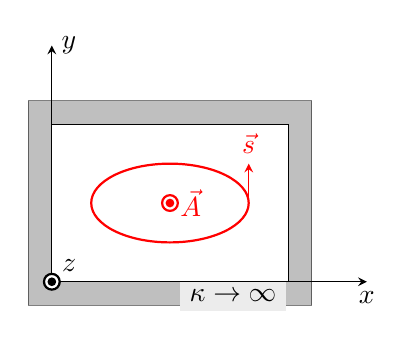
\begin{tikzpicture}
	\draw[fill=gray, opacity=0.5] (-0.3,-0.3) rectangle (3.3,2.3);
	\node[fill=lightgray!30] at (2.3,-0.18){$\kappa\to\infty$};
	\draw[thin, fill=white] (0,0) rectangle (3,2);
	\draw[thin,-stealth] (3,0) -- (4,0) node[below] {$x$};
	\draw[thin,-stealth] (0,2) -- (0,3) node[right] {$y$};
	\draw[fill=white, thick] (0,0) circle (0.1) node[anchor=south west]{$z$};
	\draw[fill=black, thick] (0,0) circle (0.04);
	\draw[red, thick] (1.5,1) circle (1 and 0.5);
	\draw[red, thin,-stealth] (2.5,1) -- +(0,0.5) node[above]{$\dd \vec{s}$};
	\draw[fill=white, thick, draw=red] (1.5,1) circle (0.1) node[anchor=west,color=red]{$\dd \vec{A}$};
	\draw[fill=red, thick, draw=red] (1.5,1) circle (0.04);
\end{tikzpicture}
	\end{center}
  Betrachtet wird ein ideal leitend berandetes Dielektrikum. Es wird zunächst davon ausgegangen, dass es eine TEM-Lösung gibt. Eine Feldlinie des Magnetfeldes müsste also (wie rot abgebildet) in der Transversalebene liegen. Sie muss sich innerhalb der Berandung schließen, weil die Ummantelung perfekt leitend ist. Diese \textbf{Randbedingung} sich mit \ref{normB} in Verbindung mit \ref{ind} begründen. Im idealen Leiter gilt, dass $\vec{E}=0$. Daraus folgt, dass auch $\rot\vec{E}=0$ und damit nach \ref{ind} auch $(\partial/\partial t) \vec{B}=0$ im im idealen Leiter null ist. Damit im idealen Leiter also ein Magnetfeld existieren kann, muss dieses zeitunabhängig sein. Im Raum propagierende elektromagnetische Wellen haben jedoch keinen Gleichanteil (der löst die Wellengleichung nicht). Folglich muss neben $E$ auch $B$ im idealen Leiter gleich 0 sein. Nach  \ref{normB} gilt $0=\vec{n}\cdot\left(\vec{B}_2-\vec{B}_1\right)$.
  Entsprechend muss die Normalkomponente des $B$ Feldes im Dielektrikum an der Grenzfläche zum idealen Leiter gleich 0 sein. Das ist gleichbedeutend damit, dass sich die Feldlinie innerhalb der Berandung schließen muss, da sie nicht aus der Ummantelung ausbrechen kann.\\
   Schaut man das Ampèreschs Durchflutungsgesetz ($\nearrow$\ref{durchf}) entlang einer beliebigen magnetischen Feldlinie an, gilt:
		\begin{equation}
			\oint\limits_{O(A)} \vec{\ubar{B}} \cdot \dd\vec{s} = \mathrm{j}\omega\varepsilon\mu \iint\limits_{A} \ubar{\vec{E}}\cdot\dd\vec{A} + \mu\iint\limits_{A} \ubar{\vec{J}}\cdot\dd\vec{A}
		\end{equation}
		Weil das Gebiet einfach zusammenhängend ist, fließt kein Strom durch die betrachtete Fläche (es gibt keinen Leiter im Dielektrikum). Das Integral über $J$ wird also 0. Gleichzeitig kann nicht sichergestellt werden, dass das Ringintegral über $B$ für alle beliebigen Integrationswege im Leiterquerschnitt gleich 0 ist.
		 Wenn das Ringintegral aber irgendwo ungleich 0 ist, muss es irgendwo eine $z$-Komponente des $E$-Feldes geben (oder die Lösung ist trivial). Das ist ein Widerspruch zur TEM-Welle.
\subsection{TE-Lösungen -- $E_z=0$}
Es wird die \(z\)-Komponente der Helmholtzgleichung für \(\vec{\ubar{H}}\) ($\nearrow$\ref{helmholtzmitgamma}) betrachtet:
	\begin{equation}
		\boxed{\left(\Delta _t + \gamma^2\right) \ubar{H}_z =  0} 
	\end{equation}
	Eine Randbedingung kann mit \ref{entkoppelgl} hergeleitet werden. Da die Berandung als idealleitend angenommen wurde (elektrisches Feld verschwindet), muss nach \ref{tanE} $\vec{E}_t\cdot\vec{t}=0$ an der Berandung gelten, wobei $\vec{t}$ ein beliebieger Tangentialvektor ist (Normalkomponenten von $\vec{E}_t$ sind zulässig, das $t$ steht hier für transversal). Das kann nur erreicht werden, wenn $\grad_t \vec{B}$ keine Normalkomponente hat. Betrachtet man nämlich eine Fläche, dann gilt, dass $\vec{n}\times\vec{t_1}=\vec{t_2}$ ist, wobei $\vec{n}$ ein Normalenvektor und $\vec{t_1}$ sowie $\vec{t_2}$ Tangentialvektoren sind. $\vu{z}$ ist aufgrund der betrachteten Leiterstruktur auf jeden Fall ein Tangentialvektor. Entsprechend muss $\grad_t \vec{B}\cdot \vec{n}=0$ sein, damit $\vec{E}_t\cdot\vec{t}=0$ nach \ref{entkoppelgl} erfüllt sein kann. Das ist nach \ref{Richtungsableitung3} gleichbedeutend mit der folgenden Randbedingung:
	\begin{equation}
		\left. \frac{\partial \ubar{H}_z}{\partial \vec{n}}\right|_{O(V)} = 0
	\end{equation}
	 Dieses \textbf{Neumannsche Randwertproblem} für $\ubar{H}_z$ kann mit den Methoden der Magnetostatik  gelöst werden. Somit erhält man eine Lösung für $\ubar{H}_z$. Weiterhin gilt \(\ubar{E}_z = 0\), somit sind die longitudinalen Komponenten bekannt. Die transversalen Komponenten lassen sich entsprechend \ref{entkoppelgl} sofort berechnen. Es gilt:
	\begin{equation}\begin{split}
		\vec{\ubar{H}}_t &= \mp \frac{\mathrm{j}}{\gamma^2}  k\, \grad _t \ubar{{H_z}}\\ 
			\ubar{\vec{E}}_t &= \pm Z\, \vu{z}\times \vec{\ubar{H}}_{t} 
		\end{split}\end{equation}		
	Damit sind die Felder im Lösungsvolumen vollständig bestimmt. Für die Feldwellenimpedanz gilt ($Z_0$ ist dabei die Feldwellenimpedanz vom TEM-Mode):	
	\begin{equation}\begin{split}	
			 \boxed{Z=\frac{\mu\omega}{ k} = \frac{ k_0}{ k}\sqrt{\frac{\mu}{\varepsilon}} = \frac{ k_0}{ k} Z_0}
	\end{split}\end{equation}
\subsection{TM-Lösungen -- $B_z=0$}
Es wird die \(z\)-Komponente der Helmholtzgleichung für \(\ubar{\vec{E}}\) ($\nearrow$\ref{helmholtzmitgamma}) betrachtet:
	\begin{equation}\label{TMGl}
		\boxed{\left(\Delta _t + \gamma^2\right) \ubar{E}_z =  0}
	\end{equation}
	 An einem idealen Leiter muss nach \ref{tanE} jede beliebige Tangentialkomponente (die \(\ubar{E}_z\)-Komponente ist in den angenommenen Leiterstrukturen transversal) verschwinden. Es resultiert die Randbedingung:
	 \begin{equation}
	 	\left. \ubar{E}_z\right|_{O(V)} = 0
	 \end{equation}
	 Das \textbf{Dirichletsche Randwertproblem} für \(\ubar{E}_z\)  kann mit den Methoden der Elektrostatik gelöst werden ($\nearrow$\ref{poilsg}). Somit erhält man eine Lösung für \(\ubar{E}_z\). Weiterhin gilt \(\ubar{B}_z=0\), somit sind die longitudinalen Komponenten bekannt. Die transversalen Komponenten lassen sich entsprechend \ref{entkoppelgl} sofort berechnen. Es gilt:
	\begin{equation}\begin{split}
		\ubar{\vec{E}}_t &=  \mp  k \frac{\mathrm{j}}{\gamma^2} \, \grad _t \ubar{E}_{z} \\
			\vec{\ubar{B}}_t = \mu\vec{\ubar{H}}_t&= -\frac{\mathrm{j}}{\gamma^2} \omega\varepsilon\mu  \vu{z}\times\grad _t \ubar{E}_{z}\\
			&= \pm \frac{\omega\varepsilon\mu}{ k} \vu{z}\times \ubar{\vec{E}}_{t} = \pm \mu \frac{1}{Z} \vu{z}\times \ubar{\vec{E}}_{t}  
	\end{split}\end{equation}
	 Damit sind die Felder im Lösungsvolumen vollständig bestimmt. Für die Feldwellenimpedanz gilt ($Z_0$ ist dabei die Feldwellenimpedanz vom TEM-Mode):
	 \begin{equation}
	 	\boxed{Z=\frac{ k}{\omega\varepsilon} = \frac{ k}{ k_0}\sqrt{\frac{\mu}{\varepsilon}} = \frac{ k}{ k_0} Z_0}
	 \end{equation}
	 \subsection{Hybride Moden}
	 Alle bisher betrachteten Moden sind Lösungen der Helmholtz-Gleichungen (lineare pDGL), die mit jeweils einem speziellen Ansatz berechnet wurden. Die Gesamtlösung im Wellenleiter ist die Superposition aus allen ausbreitungsfähigen Moden, die alle Randbedingungen erfüllt. In der Regel werden Leiter so dimensioniert, dass nur ein Mode ausbreitungsfähig ist ($\nearrow$HF), alle anderen Moden werden als Störmoden bezeichnet und sollten vermieden werden. In speziellen Anordnungen braucht man aber auch gleichzeitig TE- und TM-Mode (hybird), um überhaupt alle Randbedingungen erfüllen zu können. Dann wird die TE- mit der TM-Lösung superponiert und dann an die Randbedingungen angepasst ($\nearrow$Mikrostreifenleitung, siehe Pozar - Microwave engineering).
\subsection{Dispersionsrelation vom TM- und TE-Mode}
Beim TEM-Mode musste die Dispersionsrelation erfüllt sein ($\nearrow$\ref{disp}). Außerdem existierte er, wenn er existierte, für beliebige Frequenzen. Das ist bei TM- und TE-Moden anders! Beispielsweise muss bei TM-Moden zunächst das Randwertproblem für \(\ubar{E}_z\) gelöst werden ($\nearrow$\ref{TMGl}). Dies ist eine \textbf{Eigenwertgleichung} für die \textbf{Eigenfunktionen} \(\ubar{E}_{z\lambda}\) und den (diskreten) \textbf{Eigenwerten} \(\gamma^2_\lambda\) mit \(\lambda = 1,2,3,\ldots\). Die Eigenfunktionen werden auch \textbf{Moden} genannt und mit $\lambda$ durchnummeriert.
	\begin{equation}
		\left(\Delta _t + \gamma_\lambda^2\right) \ubar{E}_{z\lambda} =  0
	\end{equation}
	 Für eine Kreisfrequenz \(\omega\) gilt dann die Dispersionsrelation (die selbe Gleichung gilt mit analoger Herleitung auch für TE-Moden):
	 	\begin{equation}
		\gamma_\lambda^2 = \mu\varepsilon\omega^2- k_\lambda^2 \Rightarrow  k_\lambda=\sqrt{\mu\varepsilon\omega^2-\gamma_\lambda^2} \Rightarrow  \boxed{ k_\lambda=\sqrt{\mu\varepsilon}\sqrt{\omega^2-\omega_\lambda^2}}  
	\end{equation}
	Wobei $\omega_\lambda$ folgendermaßen definiert ist:
	\begin{equation}
		\omega_\lambda=\frac{\gamma_\lambda}{\sqrt{\mu\varepsilon}}
	\end{equation}
 Die \(z\)-Abhängigkeit der Lösung ist (z.B. für das elektrische Feld):
	\begin{equation}
		\ubar{\vec{E}}_\lambda(\vec{r} ) = \ubar{\vec{E}}_{0\lambda}(x,y)  \mathrm{e}^{\pm\mathrm{j} k_\lambda z}
	\end{equation}
 Für \textbf{\(\omega < \omega_\lambda\)} wird \( k_\lambda\) \textbf{imaginär} und die Lösung ist \textbf{keine propagierende Welle} mehr. Diese Lösungen sind \textbf{evaneszente Moden}:
	\begin{equation}
		\ubar{\vec{E}}_\lambda(\vec{r} ) = \ubar{\vec{E}}_{0\lambda}(x,y)  \mathrm{e}^{\mp| k_\lambda| z} \text{ für } \omega < \omega_\lambda
	\end{equation}
 Man hat also entweder ein exponentielles Wachstum oder eine exponentielle Dämpfung, wobei ersteres unphysikalisch ist. Die (Kreis)-Frequenz \(\omega_\lambda = 2\pi f_\lambda\) heißt \textbf{Cut-Off Frequenz} des Modes \(\lambda\). Die  Dispersionsrelation kann auf \( k_0=\sqrt{\mu\varepsilon}\omega\) normiert werden:
	\begin{equation}
		\frac{ k_\lambda}{ k_0}=\sqrt{1-\frac{\omega_\lambda^2}{\omega^2}}
	\end{equation}
 Dies ergibt folgendes Bild (den TEM-Mode gibt es nur, falls das Gebiet nicht einfach zusammenhängend ist):
	\begin{center}
		\begin{tikzpicture}
	\begin{axis}[
			grid=both,
			xmin = 0, xmax = 6,
			ymin = 0, ymax = 1.2,
			xtick = {0,1,2,4,4.5,5},
			xlabel = {$\omega$},
			ylabel = {$\frac{ k_\lambda}{ k}$},
			xticklabels = {0, $\omega_1$, $\omega_2$, $\omega_3$, $\omega_4$, $\omega_5$},
			width=.9\textwidth,height=.5\textwidth]
		\addplot[domain=0:6,samples=500,smooth,thick] {sqrt(1.-(1./x)^2)};
		\addplot[domain=0:6,samples=500,smooth,thick] {sqrt(1.-(2./x)^2)};
		\addplot[domain=0:6,samples=500,smooth,thick] {sqrt(1.-(4./x)^2)};
		\addplot[domain=0:6,samples=500,smooth,thick] {sqrt(1.-(4.5/x)^2)};
		\addplot[domain=0:6,samples=500,smooth,thick] {sqrt(1.-(5./x)^2)};
		\addplot[domain=0:6,samples=100,smooth,thick] {1} [yshift=8pt] node[pos=0.35] {TEM-Mode (falls nicht einfach zusammenhängend)};
		\node  at (300,25) {2 Moden (+TEM)};
	\end{axis}
\end{tikzpicture}
	\end{center}
	Von $\omega=0$ bis $\omega=\omega_1$ gibt es nur den TEM-Mode. Das ist z.B. für ein Koaxialkabel ein erstrebenswerter Frequenzbereich. Nimmt man bspw. einen Hohlwellenleiter, dann gibt es aufgrund des einfach zusammenhängenden Gebietes keinen TEM-Mode. Zwischen $\omega=\omega_1$ und $\omega=\omega_2$ gibt es dann nur einen Mode, es erstrebenswert einen Hohlleiter in diesem Frequenzbereich zu betreiben. Im Frequenzbereich zwischen $\omega=\omega_2$ und $\omega=\omega_3$ gibt es 2 ausbreitungsfähige Moden + ggf. zusätzlich den TEM-Mode. Je höher die Frequenz steigt, desto mehr Moden sind ausbreitungsfähig.
	%Gliederung sinnvoll machen, nachedem fertig geguckt
	\subsubsection{Modenentartung}
	Gerade bei Querschnitten mit \textbf{hoher Symmetrie} (z.B. quadratischer Querschnitt) kommt es dazu, \textbf{Eigenwerte übereinstimmen}. Das ist i.d.R. nicht gewollt, quadratische Querschnitte sollten nicht eingesetzt werden. Man spricht in diesem Fall von \textbf{Entartung}. In diesem Fall ergeben sich verschiedene \textbf{Eigenfunktionen} (Moden) zu identischen Grenzfrequenzen \(\omega_{\lambda_1} = \omega_{\lambda_2}\). Gibt es \(n\) Eigenlösungen zu einem Eigenwert spricht man von einer \textbf{\(n\)-fachen Entartung}. Technisch ist es sehr häufig erwünscht, nur einen ausbreitungsfähigen Mode im Arbeitsbereich zu haben (\textbf{Single-Mode-Betrieb}).
\subsection{Phasen- und Gruppengeschwindigkeiten}
\subsubsection{Phasengeschwindigkeiten} 
Die \textbf{Phasengeschwindigkeit} ist definiert als 
\begin{equation}
	v_\mathrm{p} = \frac{\omega}{ k}
\end{equation} 
	\begin{itemize}
		\item TEM-Mode \( k_0=\sqrt{\varepsilon\mu}\, \omega\):
		\begin{equation}
			v_{p0} = \frac{\omega}{ k_0} = \frac{1}{\sqrt{\varepsilon\mu}} =  v_\mathrm{c}
		\end{equation}
		\item TM/TE-Mode \( k_\lambda=\sqrt{\mu\varepsilon}\sqrt{\omega^2-\omega_\lambda^2}\):
		\begin{equation}\begin{split}
			&v_{\mathrm{p}\lambda} = \frac{\omega}{ k_\lambda} = \frac{ v_{\mathrm{p}0}}{\sqrt{1-\frac{\omega_\lambda^2}{\omega^2}}} = \frac{ v_\mathrm{c}}{\sqrt{1-\frac{\omega_\lambda^2}{\omega^2}}}\\  &v_{\mathrm{p}\lambda}(\omega\to\omega_\lambda)\to\infty \\  &v_{\mathrm{p}\lambda}(\omega\to\infty)\to v_\mathrm{c}
		\end{split}\end{equation}
	\end{itemize}
	\subsubsection{Gruppenentartung}
	Die \textbf{Gruppengeschwindigkeit} ist definiert als 
	\begin{equation}
		v_\mathrm{g} = \frac{\partial \omega}{\partial  k}
	\end{equation} 
	\begin{itemize}
		\item TEM-Mode \( k_0=\sqrt{\varepsilon\mu}\, \omega\):
		\begin{equation}
			v_\mathrm{g0} = \frac{\omega}{ k_0} = \frac{1}{\sqrt{\varepsilon\mu}} =  v_\mathrm{p0}= v_\mathrm{c}
		\end{equation}
		\item TM/TE-Mode \( k_\lambda=\sqrt{\mu\varepsilon}\sqrt{\omega^2-\omega_\lambda^2}\):
		\begin{equation}\begin{split}
			&v_{\mathrm{g}\lambda} = \frac{\partial \omega}{\partial  k_\lambda} =  v_\mathrm{c} \sqrt{1-\frac{\omega_\lambda^2}{\omega^2}} \\  &v_{\mathrm{g}\lambda}(\omega\to\omega_\lambda)=0 \\  &v_{g\lambda}(\omega\to\infty)\to v_\mathrm{c}
		\end{split}\end{equation}	
	\end{itemize}

